\documentclass{article}
\usepackage[utf8]{inputenc}
\usepackage{natbib}
\usepackage{graphicx}
\usepackage{vmargin}
\usepackage{hyperref}
\usepackage{booktabs}
\usepackage{multirow}
\usepackage{siunitx}
\setpapersize{A4}
\setlength{\parskip}{\baselineskip}%
\setlength{\parindent}{0pt}%

\title{Entregable Discretización}
\author{Laura Rodríguez Navas \\ rodrigueznavas@posgrado.uimp.es}
\date{Marzo 2020}

\begin{document}
	
\maketitle

Para la realización de este entregable se utiliza la herramienta \href{https://www.cs.waikato.ac.nz/ml/weka/}{WEKA}.

\section*{Exploración de datos}

Consideramos la base de datos \href{https://archive.ics.uci.edu/ml/datasets/Statlog+(Vehicle+Silhouettes)}{vehicle} definida sobre 18 variables predictivas (todas numéricas) y una variable clase multiclase \{opel, saab, bus, van\}. La base de datos está formada por 846 registros y en ella no existen valores desconocidos. Además, no está ordenada en función de la variable clase, es decir, la base de datos se encuentra aleatorizada. 

Con estas características, podemos proceder a la clasificación.

\section*{Clasificación}

Se usan los algoritmos de aprendizaje supervisado kNN (k=1 y k=3) y MultiLayer Perceptron en una validación cruzada de 5 carpetas (5cv) sobre la base de datos, obteniendo así una medida inicial que intentaremos mejorar con tres métodos de discretización que seleccionaremos. 

La elección de probar k=1 y k=3 con el algoritmo kNN es para ver si podemos obtener una mejor clasificación inicial con k=3 respecto k=1. Ya que con k=3 podemos reducir un poco el efecto de ruido, pero no demasiado, porqué con un valor de k más grande podría crear límites entre clases parecidas. La exactitud del algoritmo kNN puede ser severamente degradada por la presencia de ruido o características irrelevantes

La tabla siguiente refleja los resultados de las primeras clasificaciones sin incluir métodos de discretización.

\begin{center}
	\begin{tabular}{ |c|c|c| } 
		\hline
		Clasificador & Acc. en \% & ERR en \% \\
		\hline
		kNN (k=1) & 69.5035 & 30.4965 \\ 
		kNN (k=3) & 70.6856 & 47.7778 \\ 
		MultiLayer Perceptron & 81.6785 & 18.3215 \\ 
		\hline
	\end{tabular}
\end{center}

Como podemos observar, se han considerado dos parámetros de rendimiento para la evaluación de los resultados antes y después de utilizar los métodos de discretización. Estos parámetros son: los registros clasificados correctamente (Accuracy en \%) y los registros no clasificados correctamente (Error Rate en \%). 

A partir de la tabla anterior, vemos que no hemos tenido una clasificación muy buena, pero se puede mejorar. Observamos que el algoritmo kNN con k=3 es mejor clasificador que con k=1, ya que se ha podido reducir un poco el efecto de ruido. Así que, nos quedaremos con el algoritmo kNN con k=3 para la discretización. Y en comparación con el algoritmo MultiLayer Perceptron, vemos que es este mejor clasificador.

\section*{Discretización}

Las mejoras se basan en tres algoritmos de discretización: intervalos de igual amplitud, intervalos de igual frecuencia y MDLP. Es decir, dos métodos no supervisados (intervalos de igual amplitud i intervalos de igual frecuencia) y un método supervisado (MDLP).

En los métodos no supervisados (no utilizan información de las clases), los intervalos continuos se dividen en subintervalos por el parámetro especificado por el usuario (el número de bins). Por ejemplo, en el método de igual amplitud, especificando el rango de valores, y en el método de igual frecuencia, especificando el número de registros en cada intervalo.

El método supervisado (utiliza información de las clases) seleccionado se basa en la entropía.

\subsection*{Intervalos de igual amplitud}

Este método es el método de discretización sin supervisión más simple que usa intervalos iguales (binning). Determina los valores mínimo y máximo del atributo discretizado y luego divide el rango en el número definido por el usuario de intervalos discretos de igual amplitud. No hay un "mejor" número de bins, y diferentes tamaños de bins pueden revelar diferentes características de los datos. La siguiente tabla contiene los valores de precisión y tasa de error que dependen del número de bins utilizados. Se utilizaron los bins: 2, 4, 5, 10.

\begin{center}
	\begin{tabular}{cSSSSS}
		\toprule
		\multirow{2}{*}{\# of bins} &
		\multicolumn{2}{c}{kNN (k=3)} &
		\multicolumn{2}{c}{MultiLayer Perceptron} \\
		& {Acc. in \%} & {ERR in \%} & {Acc. in \%} & {ERR in \%} \\
		\midrule
		2 & 57.2104 & 42.7896 & 55.9102 & 44.0898 \\
		4 & 62.2931 & 37.7069 & 65.13 & 34.87 \\
		5 & 68.0851 & 31.9149 & 66.9031 & 33.0969 \\
		10 & 71.513 & 28.487 & 71.3948 & 28.6052 \\
		\bottomrule
	\end{tabular}				
\end{center}

\begin{center}
	\begin{tabular}{cSSSSS}
		\toprule
		\multirow{2}{*}{Clasificador} &
		\multicolumn{2}{c}{Antes Disc.} &
		\multicolumn{2}{c}{Después Disc.} \\
		& {Acc. in \%} & {ERR in \%} & {Acc. in \%} & {ERR in \%} \\
		\midrule
		kNN (k=3) & 70.6856 & 47.7778 & 71.513 & 28.487 \\
		MultiLayer Perceptron & 81.6785 & 18.3215 & 71.3948 & 28.6052 \\
		\bottomrule
	\end{tabular}
\end{center}

No es una buena discretización para estos algoritmos de aprendizaje. Sí que mejora el algoritmo kNN pero con muchos intervalos. Aún así, descartamos esta mejora ya que tener muchos intervalos nos lleva a un proceso de aprendizaje más lento e inefectivo.

\subsection*{Intervalos de igual frecuencia}

Este es otro método no supervisado, que divide los valores ordenados en k intervalos para que cada intervalo contenga aproximadamente el mismo número de registros. Por lo tanto, cada intervalo contiene n/k (posiblemente duplicados) valores adyacentes. Aquí k representa el número de bins. En el binning de igual frecuencia, se coloca un número igual de valores continuos en cada bin. La siguiente tabla contiene los valores de precisión y tasa de error que dependen del número de bins utilizados. Se utilizaron los bins: 2, 4, 5, 10.

\begin{center}
	\begin{tabular}{cSSSSS}
		\toprule
		\multirow{2}{*}{\# of bins} &
		\multicolumn{2}{c}{kNN (k=3)} &
		\multicolumn{2}{c}{MultiLayer Perceptron} \\
		& {Acc. in \%} & {ERR in \%} & {Acc. in \%} & {ERR in \%} \\
		\midrule
		2 & 61.5839 & 38.4161 & 61.1111 & 38.8889 \\
		4 & 67.9669 & 32.0331 & 71.2766 & 28.7234 \\
		5 & 68.5579 & 31.4421 & 69.1489 & 30.8511 \\
		10 & 69.6217 & 30.3783 & 71.1584 & 28.8416 \\
		\bottomrule
	\end{tabular}				
\end{center}

\begin{center}
	\begin{tabular}{cSSSSS}
		\toprule
		\multirow{2}{*}{Clasificador} &
		\multicolumn{2}{c}{Antes Disc.} &
		\multicolumn{2}{c}{Después Disc.} \\
		& {Acc. in \%} & {ERR in \%} & {Acc. in \%} & {ERR in \%} \\
		\midrule
		kNN (k=3) & 70.6856 & 47.7778 & 69.6217 & 30.3783 \\
		MultiLayer Perceptron & 81.6785 & 18.3215 & 71.1584 & 28.8416 \\
		\bottomrule
	\end{tabular}
\end{center}

La discretización en intervalos de igual amplitud produce más desequilibrios que la discretización en intervalos de igual frecuencia, ver figuras \ref{fig:igual_amplitud} y \ref{fig:igual_frecuencia}. Aun así, la discretización en intervalos de igual frecuencia no es una buena discretización para estos algoritmos de aprendizaje. Hasta es peor.

Sabemos que existe una relación directa entre los métodos de aprendizaje no supervisado y los métodos de discretización no supervisados. Lo mismo entre los métodos de aprendizaje supervisado y los métodos de discretización supervisados. Como consecuencia, generalmente los métodos de discretización no supervisados son más adecuados para algoritmos de aprendizaje no supervisados. Y los métodos de discretización supervisados son más adecuados para algoritmos de aprendizaje supervisados.

En este caso, podríamos llegar a la conclusión que los métodos de discretización no supervisados seleccionados no son buenos para los algoritmos de aprendizaje supervisados kNN y MultiLayer Perceptron basándonos en el comentario anterior.

\begin{figure}[h]
	\centering
	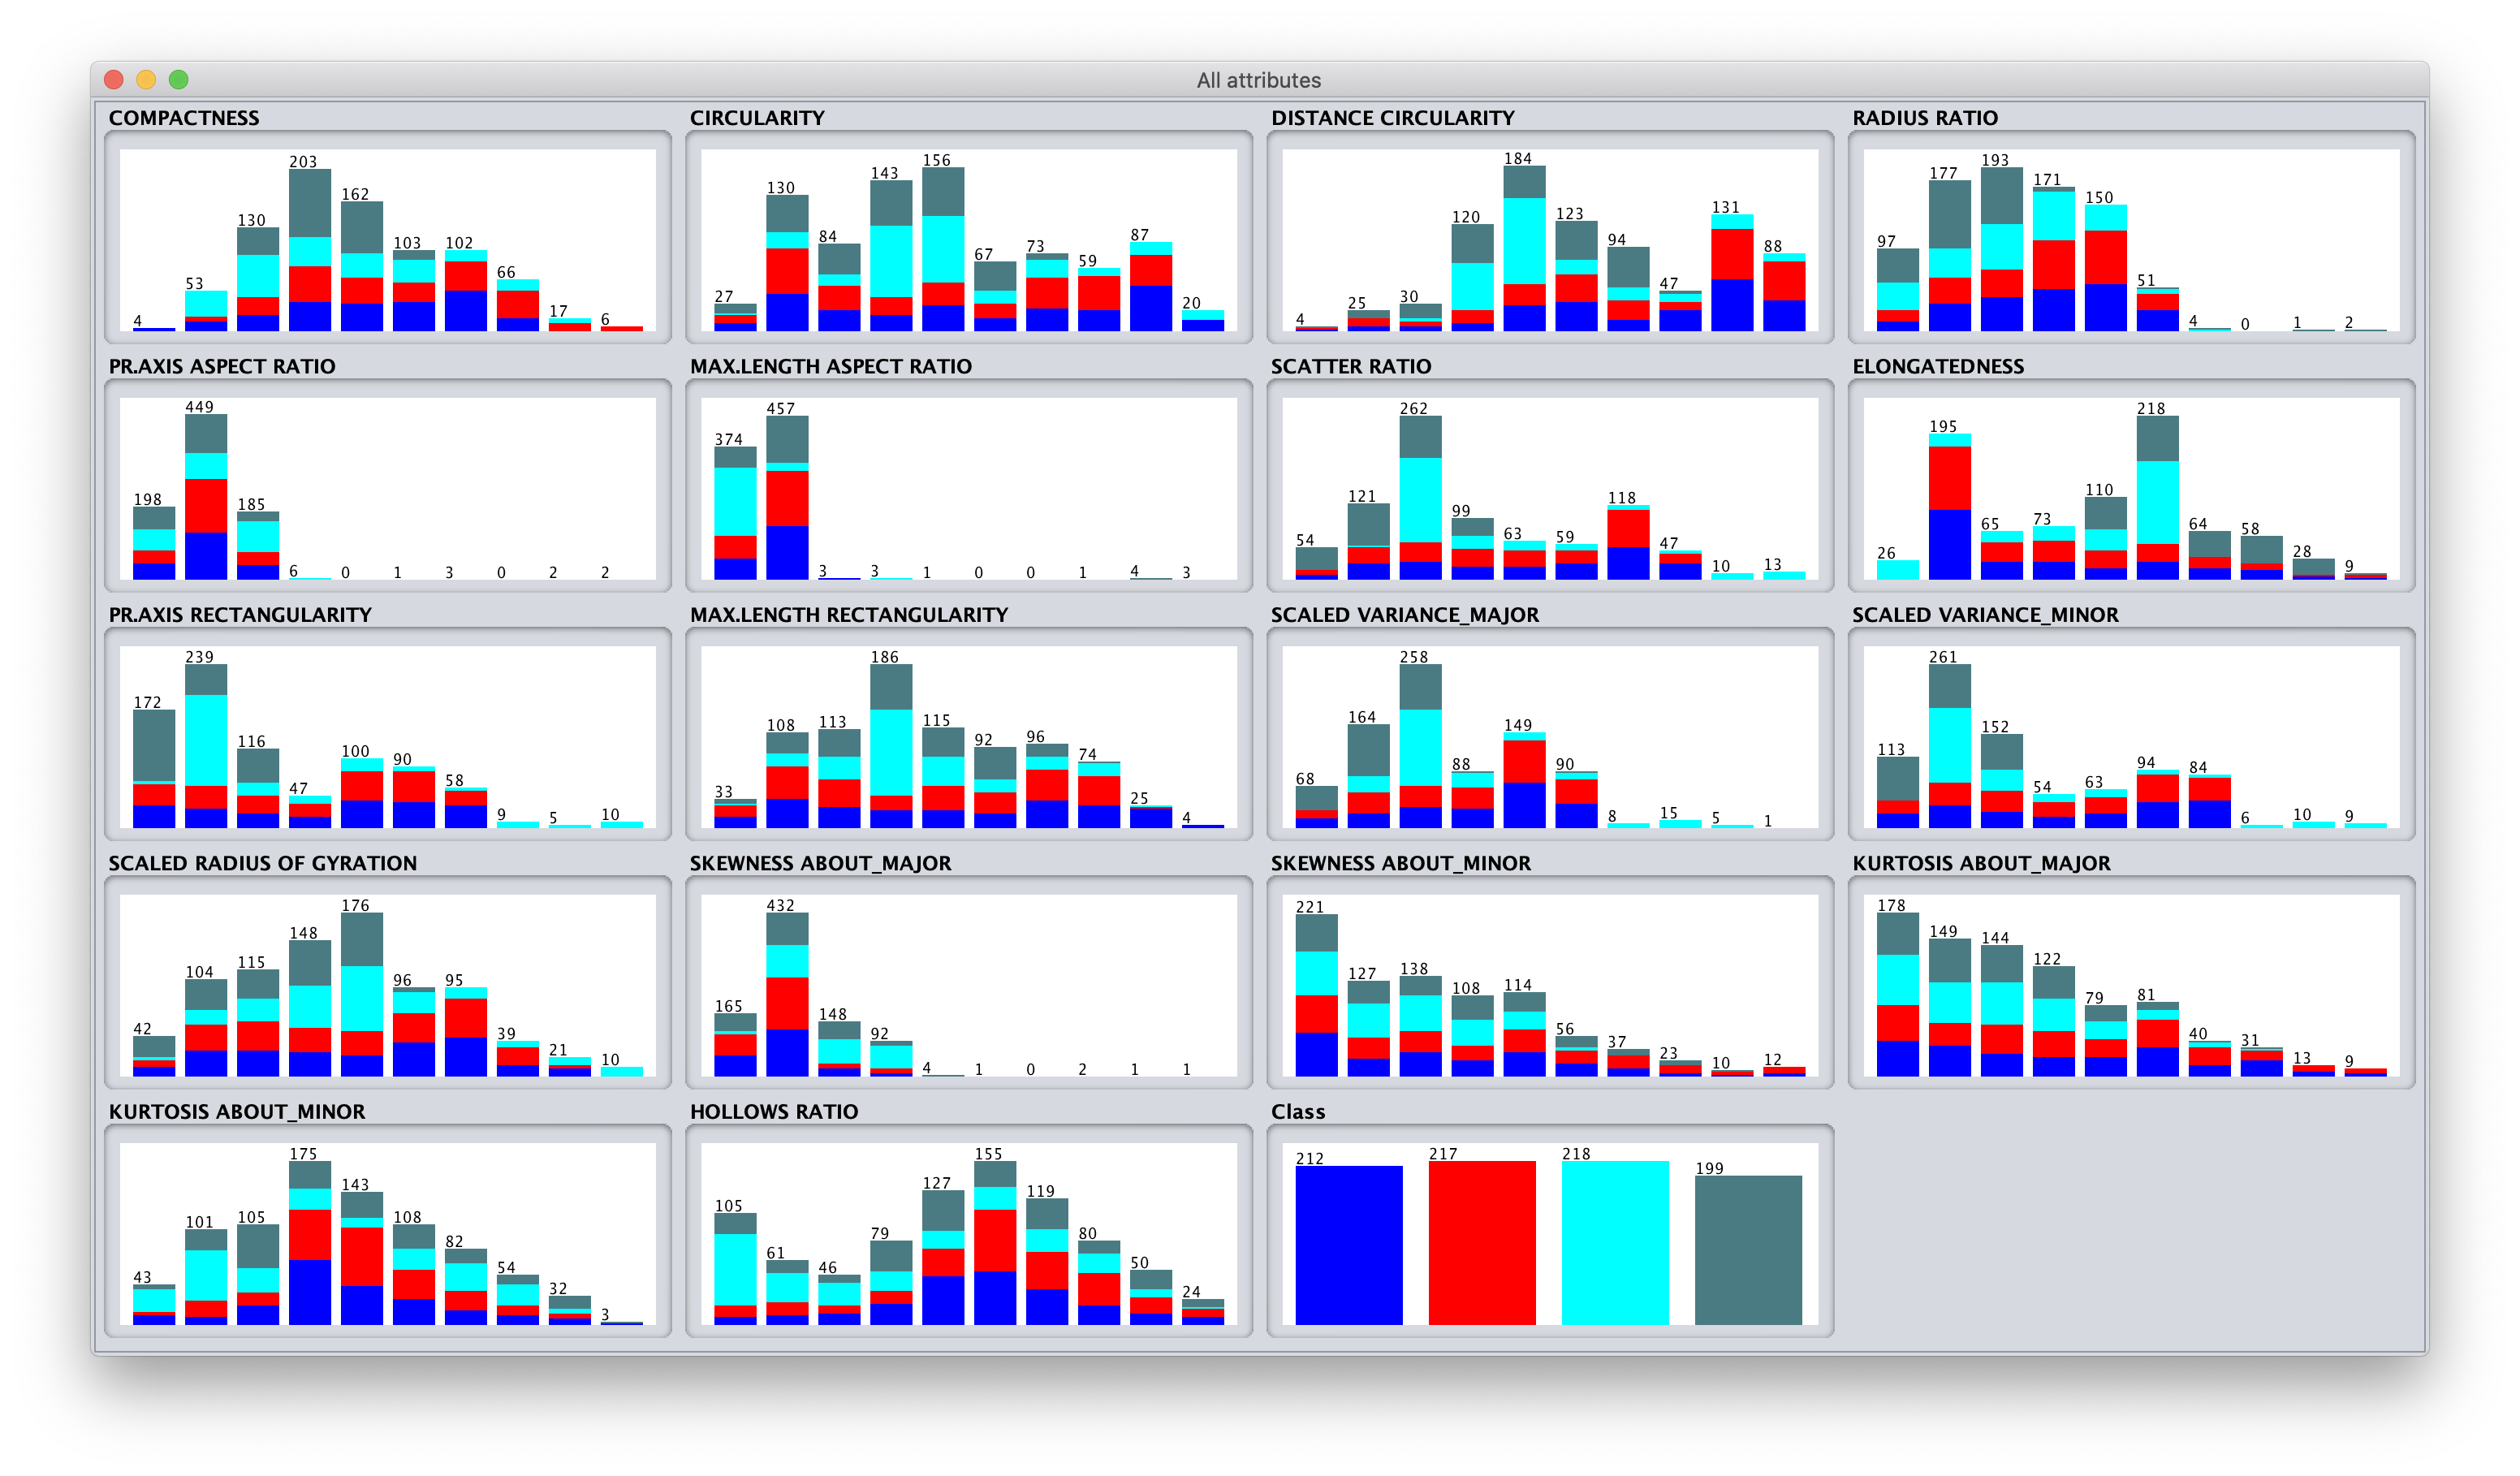
\includegraphics[width=0.6\textwidth]{igual_amplitud.png}
	\caption{intervalos de igual amplitud.}
	\label{fig:igual_amplitud}
\end{figure}

\begin{figure}[h]
	\centering
	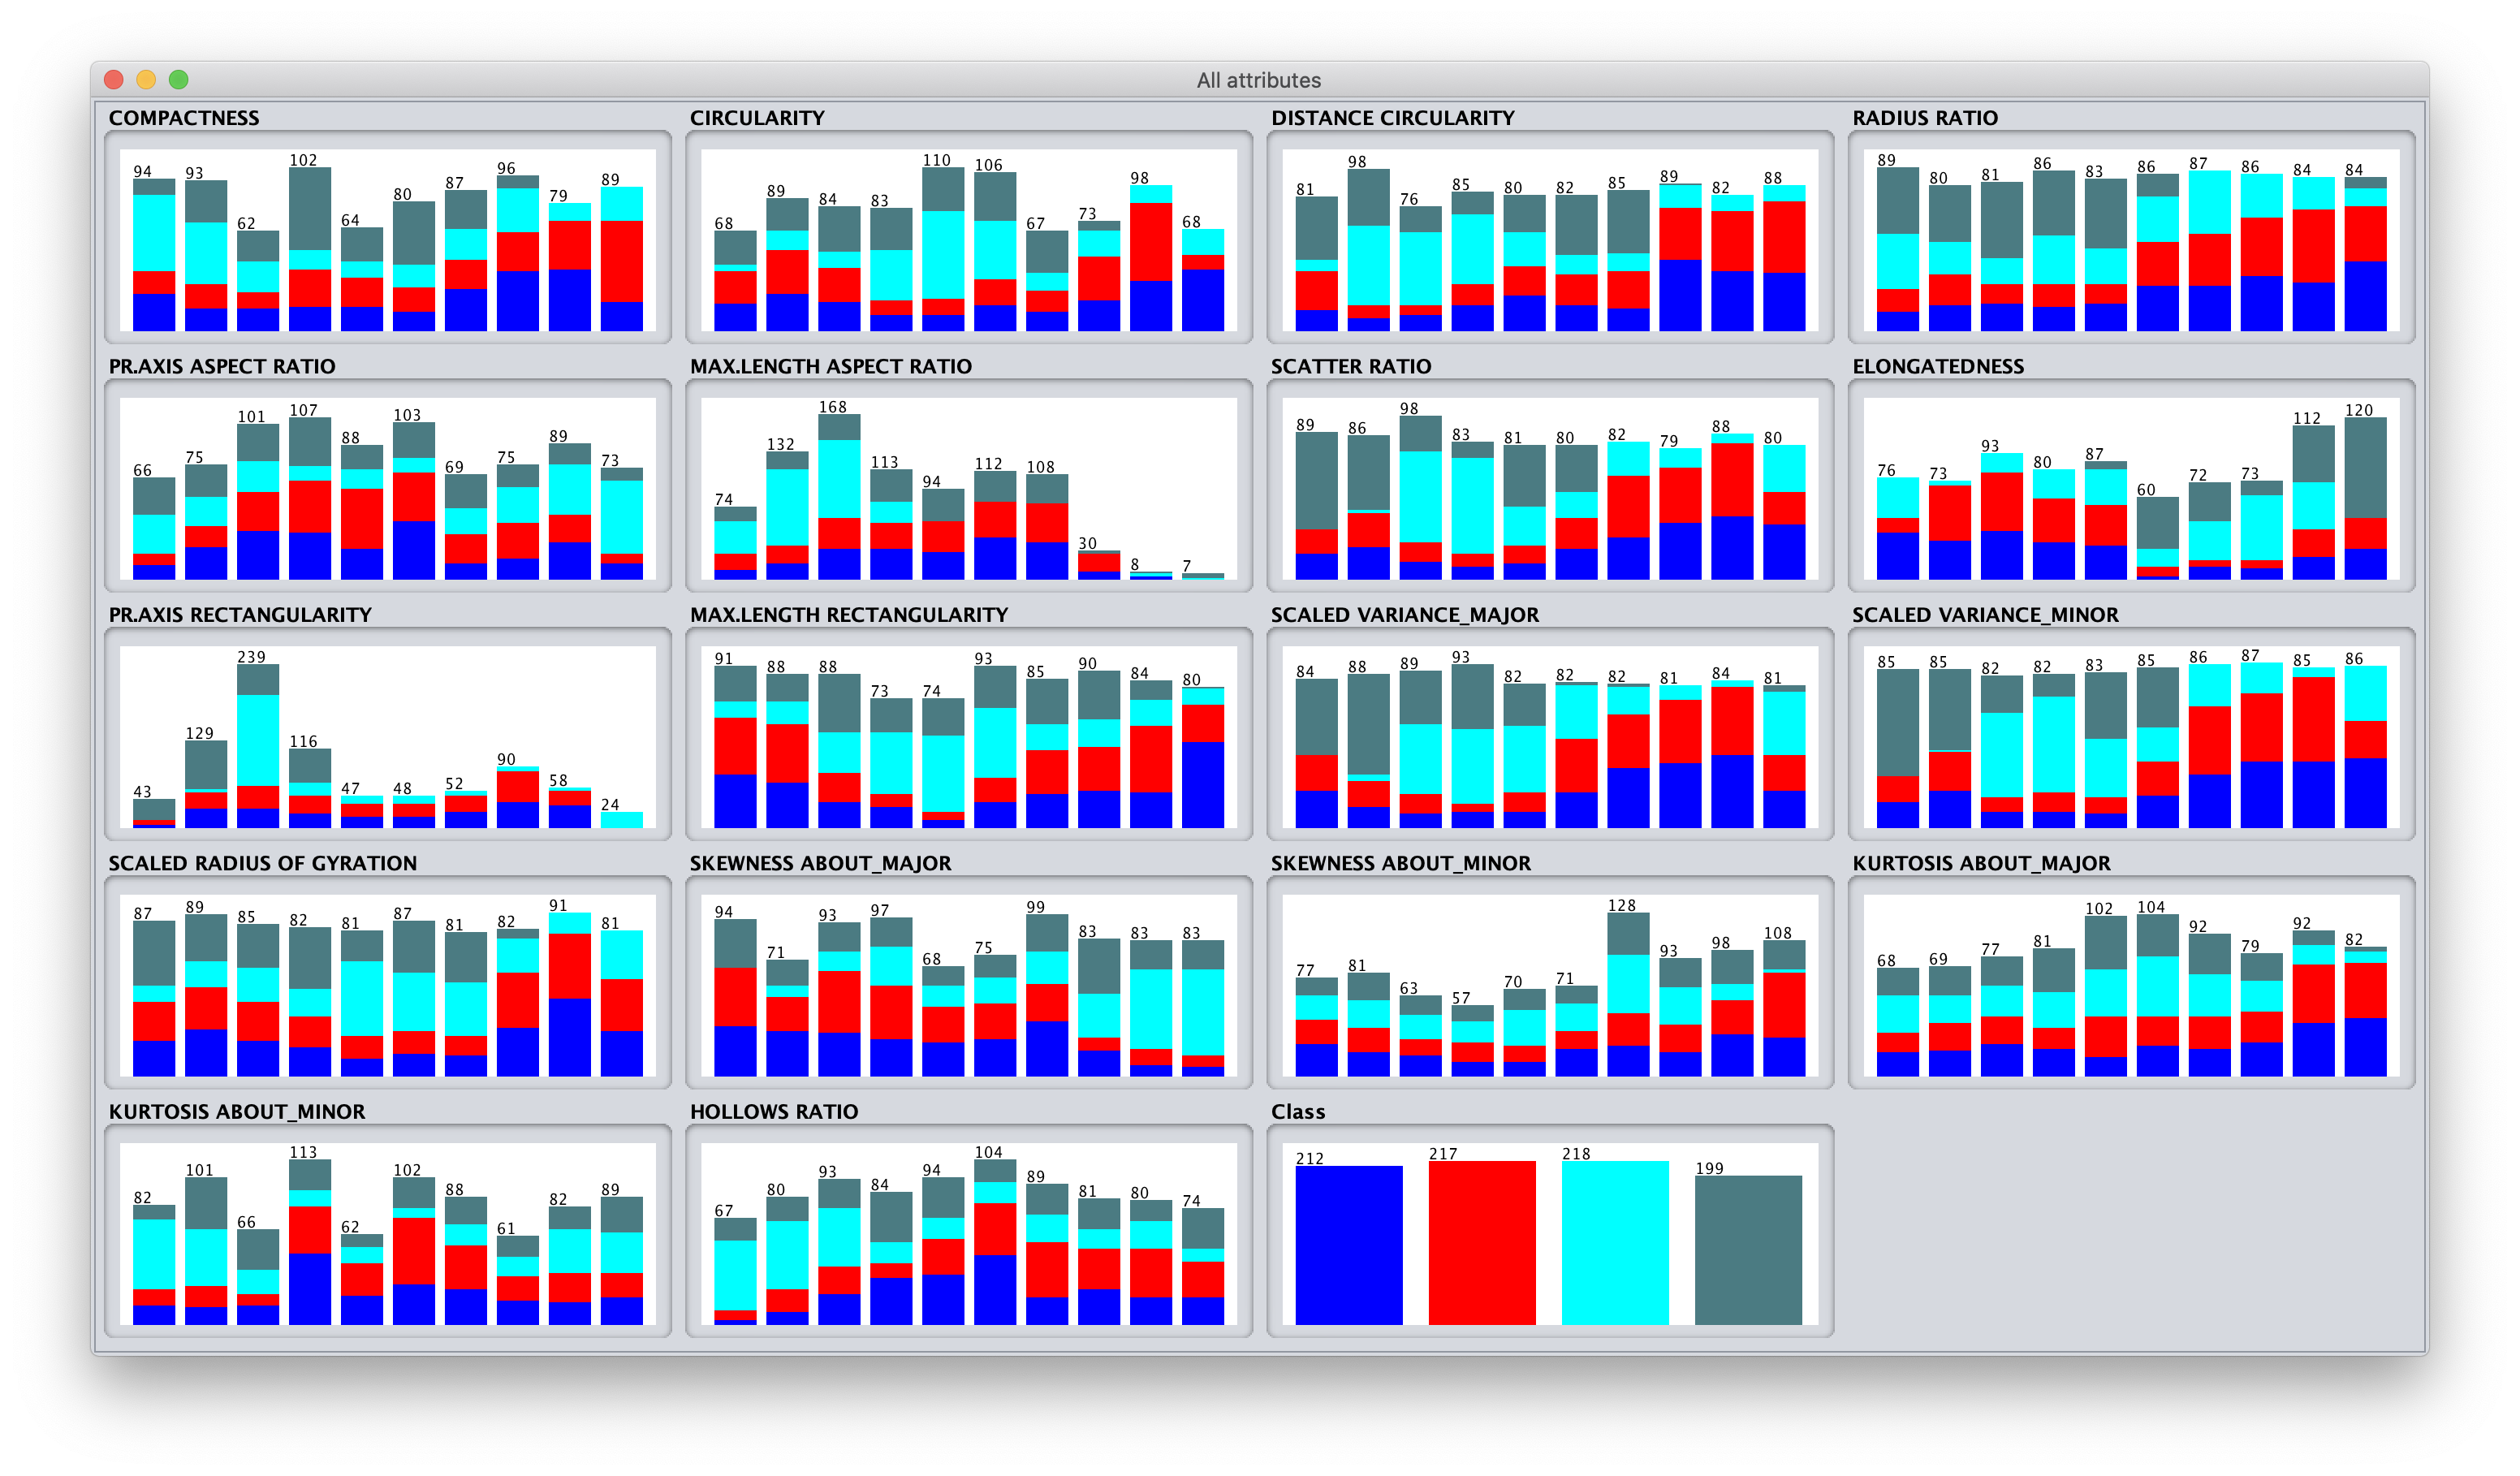
\includegraphics[width=0.6\textwidth]{igual_frecuencia.png}
	\caption{intervalos de igual frecuencia.}
	\label{fig:igual_frecuencia}
\end{figure}

\subsection*{MDLP}

El método de discretización supervisado MDLP, o también conocido como el método de Fayyad, es un método de división que va dividiendo progresivamente el dominio continuo de cada variable. Se basa en la medida de la entropía que considera la variable clase para evaluar cada uno de los posibles intervalos. Además, aplica el principio de la longitud de descripción mínima para ir escogiendo esos intervalos.

Como característica importante, tiene como parámetro de entrada el número máximo de intervalos. Esto evita que se cree un número elevado de intervalos y hace augmentar la posibilidad de mejoras, ya que tener muchos intervalos nos lleva a un proceso de aprendizaje más lento e inefectivo.

A continuación los resultados,

\begin{center}
	\begin{tabular}{cSSSSS}
		\toprule
		\multirow{2}{*}{Clasificador} &
		\multicolumn{2}{c}{Antes Disc.} &
		\multicolumn{2}{c}{Después Disc.} \\
		& {Acc. in \%} & {ERR in \%} & {Acc. in \%} & {ERR in \%} \\
		\midrule
		kNN (k=3) & 70.6856 & 47.7778 & 73.4043 & 26.5957 \\
		MultiLayer Perceptron & 81.6785 & 18.3215 & 71.0402 & 28.9598 \\
		\bottomrule
	\end{tabular}
\end{center}

Es una buena discretización para el algoritmo kNN. Pero no es una buena discretización para el algoritmo MultiLayer Perceptron, porqué las discretizaciones son críticas en métodos de inducción de reglas como MultiLayer Perceptron.

Como conclusión, respecto al ratio de inconsistencia, vemos que casi todos los tres métodos analizados tienen una tendencia similar con menor ratio. Podría deberse a que se han utilizado los datos del conjunto de entrenamiento a la hora clasificar.


\end{document}
